\documentclass[12pt]{article}
\usepackage[utf8]{inputenc}
\usepackage{amssymb}
\usepackage{amsmath}
\usepackage{graphicx}

\title{AI1110 ASSIGNMENT-1}
\author{CS21BTECH11024 - Jonnala Varshini}

\begin{document}
\maketitle
\section*{ICSE 10 2018}
\section*{Question 7(c)}
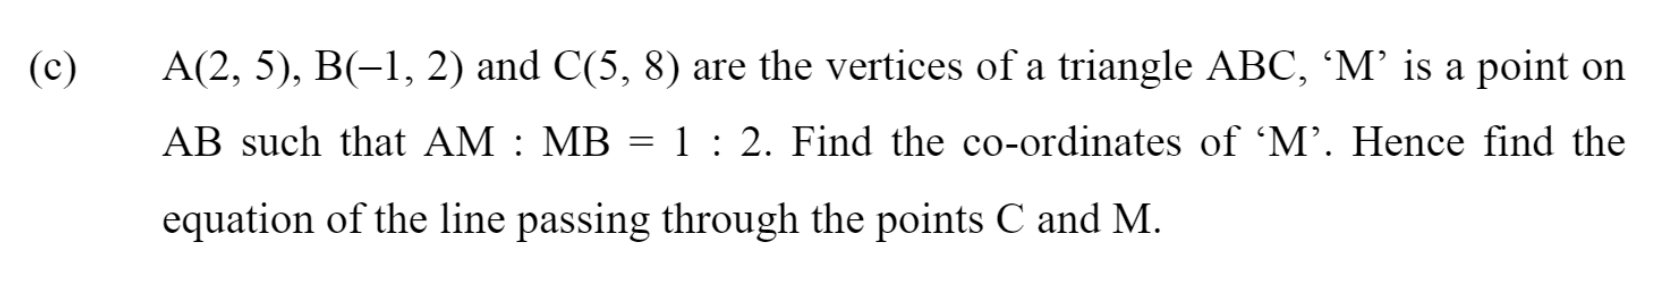
\includegraphics[width=\textwidth]{prv1a.png}
\section*{Solution:}
According to the question, $M$ is a point on the side $AB$ such that $$AM : MB = 1 : 2$$
It is known that, \\
    When the line segment AB is divided internally by C in the ratio m:n,\\
we use Section formula to find the point C.\\\\
The Coordinates of point C will be,
  [$\frac{mx2+nx1}{m+n}$, $\frac{my2+ny1}{m+n}$], where $A(x1,y1)$,$B(x2,y2)$ \\\\
From given data, using Section formula, we get\\\\
    $M$ = ($\frac{-1+4}{1+2}$,$\frac{2+10}{1+2}$) = $(1,4)$\newpage
The equation of the line joining two points (a,b),(c,d) is \\
        (y-b) = {$\frac{d-b}{c-a}$}(x-a)\\\\
Here, the equation of the line joining $C(5,8)$ and $M(1,4)$ will be\\
      (y-4) = $\frac{8-4}{5-1}$(x-1) \\\\
Simplified, we get the equation $$x-y+3=0$$
\subsection*{But, However,} On calculating, we get\\
The equation of the line joining $A(2,5), B(-1,2)$ as $x-y+3=0$ and \\
the equation of the line joining $B(-1,2), C(5,8)$ as $x-y+3=0$ too.\\
This implies that A,B,C are `collinear' and pass through $x-y+3=0$ and hence, given points $A,B,C$ don't form a triangle.\newline
Verifying by plotting the graph of A,B,C and M points :
\begin{center}
  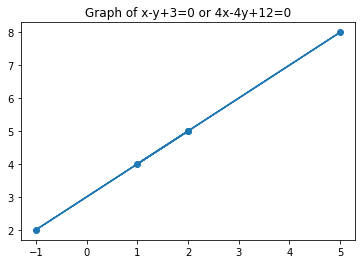
\includegraphics[width=\textwidth]{prv1b.png}
\end{center}
    
\end{document}
